% !TeX root = ../main.tex
% Add the above to each chapter to make compiling the PDF easier in some editors.

\chapter{Background}\label{chapter:background}

This chapter discusses the relevant background knowledge required to understand the remainder of this work.

\section{Trusted execution environment}

One of the core security concepts of operating systems are the privilege levels of processes. Thereby, processes are protected against other processes with the same or lower privilege level. However, they are not protected against more privileged processes. This bears problems for example for cloud computing and edge computing. In cloud computing, other services, the hypervisor, or the cloud provider in general could potentially access sensitive data of the cloud tenant. In edge computing, the edge applications deal with plain text data, while they are potentially running on insecure edge devices. Hence, protection against more privileged processes is desired.

% Global Platform = industry standard

A \ac{TEE} is an integrated hardware extension to processors. Effectively, the execution environment is separated into the \ac{REE} and the \ac{TEE} by hardware. The \ac{REE} runs the common software, e.g., a Linux-based operating system and the user applications.
The TEE is an isolated tamper-resistant execution environment that guarantees the authenticity of the executed code, and the integrity of runtime states (e.g., memory) \cite{Sabt2015}.
Since a \ac{TEE} is integrated into the processor, there is no separate chip required.
% The TEE allows code to be executed and memory separately to be used on a device in a hardware-protected manner that ensures a high level of confidentiality and integrity.
% TODO: Which previous technologies?
Moreover, the \ac{TEE} commonly follows the same user and kernel space separation as \ac{REE} operating systems. The kernel space is running a trusted OS kernel, and the user space is running the trusted applications.

Previous technologies ensure protection of data-in-transit, and data-at-rest, while \ac{TEE} additionally protects data-in-use.
For example, smart cards are commonly used to store keys to identify users and keys to encrypt data-at-rest \cite{Arthur2015}.

One such \ac{TEE} is ARM's TrustZone~\cite{ARM09, Ngabonziza2016}. It partitions all software and hardware resources of the containing system into the \ac{NW} and the \ac{SW}.
While the \ac{SW} can access the resources of the \ac{SW} and the \ac{NW}, the \ac{NW} is restricted to its own resources.
Since ARM is the dominant processor architectures for IoT devices with a market share of 86\,\% \cite{eclipse}, many of the approaches in this field of research rely on ARM technology such as TrustZone.
Our approach also leverages TrustZone to enable the execution and the remote attestation of an fTPM.

Other \ac{TEE} technologies are Intel Software Guard Extensions~(SGX), and AMD Secure Encrypted Virtualization~(SEV), in the future also Intel Trusted Domain Extensions~(TDX), and ARM Confidential Computing Architecture~(CCA). Since we focus on the implementation of our concept with ARM TrustZone, we do not go into detail about these other technologies here. However, since our concept is not tied to ARM processors and can also be applied to others, they are mentioned for the sake of completeness.

% TrustZone, Trusted applications are not isolated -> they need to trust each other

% static: ARM TZ
% dynamic: Intel SGX, TDX, AMD SEV


\section{Attestation}

According to the Cambridge Dictionary an attestation is ``a formal statement that you make and officially say is true''.
% Cite with biber?
Specifically in our context, attestation is a mechanism for software to prove its identity.
In the following, the two types are discussed.


\subsection{Local attestation}

Local attestation enables assertions between two environments on the same system \cite{Anati2013InnovativeTF}. The claim of an environment can be verified by another environment, usually with the help of message authentication codes (MAC) \cite{Menetrey2022}. For example, Intel SGX uses this mechanism to establish assertions between two enclaves \cite{Anati2013InnovativeTF}.

\subsection{Remote attestation}

\begin{figure}[htpb]
  \centering
  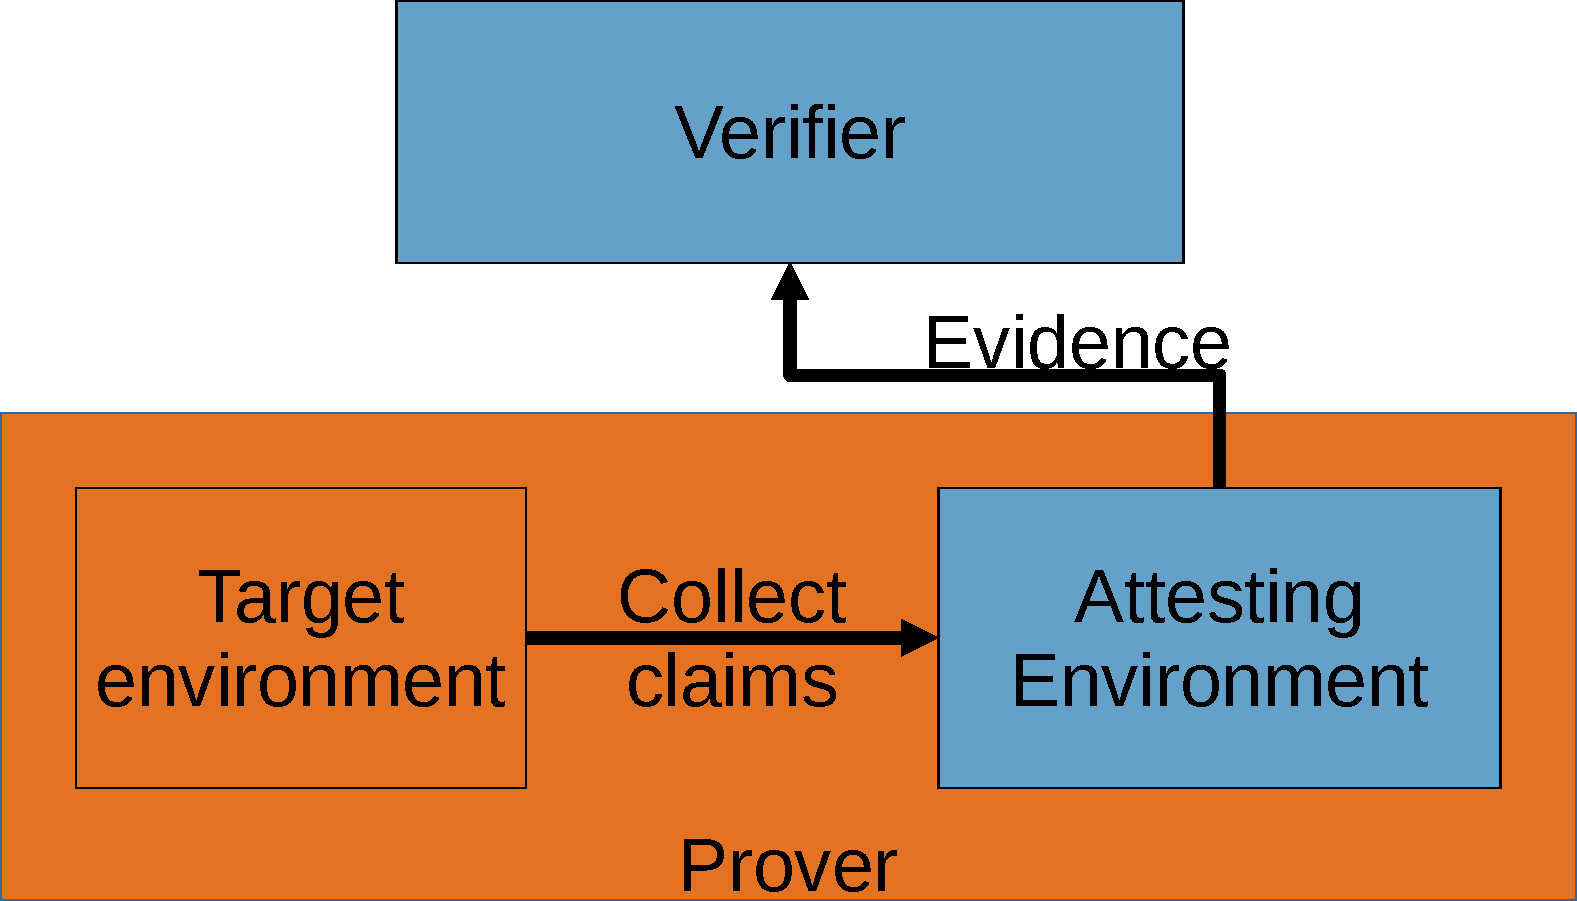
\includegraphics[trim={0 5cm 0 0}, width=0.5\linewidth]{figures/remote_attestation.pdf}
  \caption{Data flow of remote attestation \cite{rfc9334}. Initially, only the blue areas are trusted by the verifier. After the attestation, the verifier also trusts the target environment.} \label{fig:ra}
\end{figure}

Remote attestation is a challenge-response protocol initiated by a remote attestor. \autoref{fig:ra} depicts a simplified overview of the data flow of a remote attestation.
The process is initiated by a remote trusted party (called ``verifier'') to verify that a target environment on the end-device (called ``prover'') has not been tampered with \cite{Menetrey2022, Coker2011}. This challenge contains a nonce, enforcing a fresh response.
The response must be an evidence of the challenged system that it is trustworthy. To build that, an attesting environment on the prover device generally inspects the following properties of a program: (i) its code and data has been correctly loaded into memory for execution, and (ii) its data has not been maliciously modified at runtime.

The attesting environment acts as a trust anchor for the verifier.
A trusted anchor is required on the device to be attested because at least one trusted component is necessary to extract the data from the remote device to be verified. In many cases, TEE's act as a trust anchor because they are hardware-protected, making it an excellent candidate for a trust anchor.

\section{Trusted Platform Module}

The \ac{TCG} published the first TPM specification (v1.2) in 2009 \cite{ISO11889}, and the most current specification (v2.0 Revision 01.59) ten years later in 2019 \cite{tpm}.
% First v2.0 version was much earlier
It describes a cryptographic coprocessor that increases trust in the host platform. Specifically, this means that the platform exhibits the expected behavior and that this behavior can be trusted.
For that, the TPM maintains a separated state from the host platform, which enables the TPM to take measurements of the host platform.
It is also a passive device, meaning it only does something when prompted.
\autoref{tab:tpm_use_cases} summarizes the main features of TPMs.

\begin{table}[htpb]
  \caption[TPM features]{TPM main features and according short explanations.}\label{tab:tpm_use_cases}
  \centering
  \begin{tblr}{Q[l,m] Q[l,m]}
      \toprule
      Feature & Explanation \\
      \midrule
      Device identification    & {Identify a machine, e.g., before\\ granting it access to resources} \\
      % Encryption               & Encrypt files on a device \\
      True Random Number Generator  & Seed key generation algorithms \\
      Key Storage              & Store secret keys \\
      Platform Configuration Registers & {Store measurements of system components} \\
      Sealing                  & {Bind access to data to state of host system\\i.e., specific PCR values} \\
      \bottomrule
  \end{tblr}
\end{table}


The \ac{PCR} values are the fundament for the remote system attestation. They are one-way registers, which values can never be written to an exact value, but only be extended.
This is known as 'hash extend'.
Its properties prohibit the removal of extensions, and the arbitrary writing of values, whether by a benign or malicious actor.
The PCR value at index $i$ can only be modified (i.e., extended) in the following way:
\[ PCR(i)_0 \coloneqq 0,\quad PCR(i)_{t+1} \coloneqq hash(PCR(i)_t\ \Vert\ new\ value)\]

A PCR value holds a hash representing the platform state.
Thereby, a remote attestor can request a so-called 'quote' from the TPM on the host in question.
A quote contains the PCR values and is digitally signed.

Typically, a TPM contains 24 PCR values that form a bank, with the lower PCR values representing the system boot process and the higher ones representing the events after the kernel is booted \cite{Arthur2015}.
%\autoref{tab:pcr_usages} shows the components each PCR value represents as specified by the TPM PC Client specification \cite{tcgPcClient}.
The fixed length of the \ac{PCR} values is important for memory-constrained TPMs \cite{Arthur2015}.

%\begin{table}[htpb]
  \caption[PCR table]{The PCR register usages as defined by the TPM PC Client specification \cite{tcgPcClient}.}\label{tab:sample}
  \centering
  \begin{tblr}{Q[c,m] Q[l,m]}
      \toprule
      PCR Index & Usage \\
      \midrule
      0    & {SRTM, BIOS, host platform extensions,\\ embedded Option
      ROMs and PI Drivers} \\
      1    & Host platform configuration \\
      2    & UEFI driver and application code \\
      3    & UEFI driver and application configuration and data \\
      4    & UEFI Boot Manager code (usually the MBR) and boot attempts \\
      5    & {Boot Manager Code configuration/data and GPT/partition table} \\
      6    & Host platform manufacturer specific \\
      7    & Secure boot policy \\
      8-15 & Defined for use by the static OS \\
      16   & Debug \\
      23   & Application support \\
      \bottomrule
  \end{tblr}
\end{table}


% Sealing (local attestation)
% EKCert, EK = Unique ID, key in TPM, used for validation
% Binding to TPM (EK)
% Core Root of Trust of Measurement: BIOS extension, trusted hashing
% Attestation: TPM confirms measured state

TPM~1.2 is limited to SHA-1 hashes which are considered broken \cite{cryptoeprint:2005/010, Wang2005, Stevens2017}. Although the SHA-1 uses in TPM~1.2 were analyzed to be not affected \cite{sha1tpm12}, cryptographic algorithms only become weaker over time \cite{Arthur2015}. In reaction, TPM~2.0 offers crypto-agility and allows newer algorithms such as SHA-256. In general, TPM~2.0 is more flexible, and is always turned on, while a TPM~1.2 needed to be turned on manually. Also, TPM~2.0 is more consistent across different implementations because of broader specifications.
TPM~2.0 is the focused version nowadays, e.g., Microsoft recommends TPM~2.0 over TPM~1.2 because of security advantages \cite{micrec}, and also requires TPM~2.0 for Windows~11 with SHA-256 PCR banks \cite{win11req}.

% SRTM (from the beginning, what we use)
% DRTM (at any point of time, established by HW extensions, root of trust is e.g. Intel microcode/Hardware)

\begin{figure}[htpb]
  \centering
  \begin{subfigure}{0.49\textwidth}
    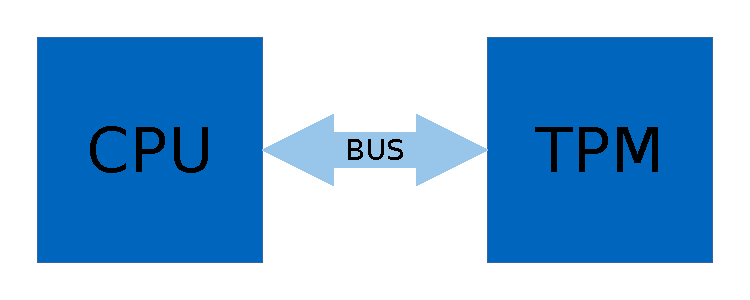
\includegraphics[width=\linewidth]{figures/dTPM.pdf}
    \caption{Discrete TPM} \label{fig:dtpm}
  \end{subfigure}%
  \hspace*{\fill}   % maximize separation between the subfigures
  \begin{subfigure}{0.49\textwidth}
    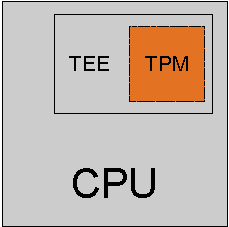
\includegraphics[width=\linewidth]{figures/fTPM.pdf}
    \caption{Firmware TPM} \label{fig:ftpm}
  \end{subfigure}%

  \begin{subfigure}{0.49\textwidth}
    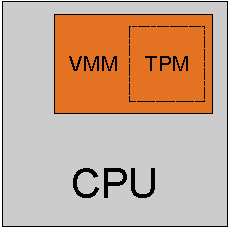
\includegraphics[width=\linewidth]{figures/vTPM.pdf}
    \caption{Virtual TPM} \label{fig:vtpm}
  \end{subfigure}%

  \caption{Schematic illustration of the different TPM types in their pure form. Blue: Hardware, Orange: Software.} \label{fig:tpm_types}
\end{figure}


There are three types of TPMs, as illustrated in \autoref{fig:tpm_types}. They all offer the same functionality, but with different security guarantees and performance characteristics.

\subsection{Discrete TPM}

This is the classical form of a TPM. It is a dedicated piece of hardware, connected to the CPU via a bus. It is designed and manufactured to be highly temper-resistant against hardware attacks.
The TPM specifications \cite{tpm, tcgPcClient} do not demand a specific bus system, however, they define the interfaces between the TPM and the following bus systems: LPC, I\textsuperscript{2}C, and SPI.

The well-known 'TPM Reset Attack' was independently described in \cite{kauerBernhard,sparks2007}. It requires minimal hardware, precisely only a wire connecting the reset line of the LPC bus \cite{lpc} to ground. This results in a reset signal for the TPM, yielding predictable values for the \ac{PCR} registers, i.e., 0. This allows an attacker to replay the measurement log of a benign boot process to achieve valid \ac{PCR} values, even though a modified chain has been booted.
Since TPM 1.2, TCG provides a mitigation specification for this reset attack \cite{tcgResetFix}, requiring the BIOS to overwrite sensitive data after each unexpected reset, preventing an attacker to gain a valid measurement log.
% TODO: That's claimed by Winter2013 but that the mitigation works because the attacker cannot gain a valid measurement log is from me. But is measurement log really sensitive? Otherwise I'm not sure how the mitigation prevents the attack, since the spec only changes the behavior of the platform on reset, not the TPM on reset. And with the upper described attack, only the TPM is reset.
However, this mitigation is still vulnerable to cold boot attacks \cite{Halderman2009, Winter2013}.

Winter and Dietrich \cite{Winter2013} demonstrate a bus modification attack at TPMs integrated with the LPC bus or the I\textsuperscript{2}C bus.
Their approach, labeled 'Active LPC frame hijacking', allows them to "lift" commands to a higher locality than the one they were originally sent with. This allows them to evolve the 'TPM Reset attack' from being only usable for S-RTM, to also D-RTM systems.
They also introduce a new approach of circumventing the TPM's measurement feature. Instead of resetting the TPM as previously described \cite{kauerBernhard,sparks2007}, they reset the main device, i.e., the users' device like a desktop PC while preventing the TPM from receiving the reset signal. This keeps the state of the TPM, e.g., the valid \ac{PCR} values of the previous boot procedure, and the attacker can hijack the boot procedure triggered by the platform's reset and boot a malicious operating system or firmware, while the TPM still stores the old and valid PCRs. While its conceptually easier since the attacker does not need to know the measurement log since the valid \ac{PCR} values are already in-place, it requires active manipulation of bus transmissions to shield the TPM from the reset signal.

Seunghun Han et al. \cite{aBadDream} report two attacks on discrete TPMs to reset the PCR registers. The first targets a gray area in the power management section of the TPM 2.0 specification. The TPM shall store its state into the (its?) non-volatile random access memory (NVRAM) before shutting down when the host platform goes to sleep, and restore it when it wakes up. However, the specification is missing a concrete description how to handle a lack of a stored state when waking up. Therefore, some implementations simply reset the state. Their second attack targets a DRTM, namely an implementation flaw in tboot \cite{tboot}, the most widely used measured boot environment used with Intel's Trusted Execution Technology. However, in their work, they found that some mutable function pointers are not measured, which allows attacks.

A time-based side-channel attack \cite{Moghimi2019} during signature generation based on elliptic curves allows an attacker to recover 256-bit private keys for ECDSA and ECSchnorr signatures.

A passive sniffing attack is shown in \cite{Kursawe2005AnalyzingTP}. It is applicable to TPM 1.1 connected to an LPC bus. They observed that the data of some operations like unsealing are transmitted via the bus in plain text. Since TPM 1.2, however, the modules no longer send sensitive data unencrypted \cite{Winter2013}.

That invasive hardware attacks against dTPMs are possible was already shown by Tarnovsky in 2010 \cite{tarnovsky}. However, this requires a lot of time, knowledge and resources, i.e., hardware and money.


\subsection{Firmware TPM}

% Generally more secure? According to https://arxiv.org/pdf/2304.14717.pdf, yes
% But TEEs are also tamper-resistant, aren't they? Maybe not as much as dTPMs.

As seen in the previous section about discrete TPMs, the bus between the CPU and a TPM can be considered as their biggest attack vector. An fTPM \cite{Raj2015, 197213} circumvents this by being directly executed within the CPU within a \ac{TEE}, revealing no easily accessible bus.
The trend is moving towards fTPMs, which can also been seen by the increasing efforts to bring an fTPM to the RISC-V processor family \cite{Boubakri2021}. Also, since they require less hardware, they are cheaper for manufacturers.

Cheng et al. \cite{Cheng2020} conducted a detailed performance comparison between dTPMs and fTPMs. They found that fTPMs are faster overall. %, but especially in key loading, sealing, unsealing, signature verification, and encryption.
In addition, as is the nature of software, fTPMs are easier to update than dTPMs.

However, there are also disadvantages. First, they cannot provide true RNG, since hardware is required for that. Second, they are started later in the boot chain than a dTPM that is accessible from the beginning. This has the consequence that the hashes of the preceding boot components cannot be sent to the fTPM. Last, fTPMs depend on more components for its security than single-component dTPMs, e.g., the \ac{TEE}, and the boot chain.

Of course, there are also attacks against fTPMs.
The previously mentioned side-channel attack \cite{Moghimi2019} against dTPMs, can also be applied to fTPMs.

Jacob et al. \cite{Jacob2023} target proprietary AMD fTPMs by attacking their \ac{TEE}, namely the AMD Secure Processor~(AMD-SP). Thereby, they can expose the full internal state of the fTPM bypassing any authentication mechanisms. To do so, they leak the secret key from the BIOS flash chip which is used to derive the encryption and signature keys for the fTPMs non-volatile data. They achieve this by using a voltage fault injection that bypasses the authenticity check in the boot process and allows them to boot their own firmware component that leaks the required information.

% \begin{table}[htpb]
%   \caption[ftpmdownsides]{Advantages and disadvantages of fTPMs.}\label{tab:tpm_comparison}
%   \centering
%   \begin{tblr}{Q[l,h] Q[l,m]}
%     \toprule
%     Advantages      &  Disadvantages \\
%     \midrule
%     Faster          &  No perfect RNG \\
%     Easier update   &  {Launched later in boot chain.\\ Cannot measure hashes of preceding boot components.} \\
%     \bottomrule
%   \end{tblr}
% \end{table}


\subsection{Virtual TPM}

% Confidential Computing approaches (Fraunhofer paper), our solution could be a use-case for that

% Provided by hypervisor (not necessarily, I read a paper which does not need to trust hypervisor. Don't remember what provides it.)


\section{Secure Boot and Measured Boot}

Secure boot is a concept of UEFI doing local attestation of components directly at boot-time. Based on signatures of next-to-boot components. It cancels the boot process as soon as deviations are detected. Binaries of components are first signed and then, deployed universally. Hence, binaries are not bound to the platform and can be considered portable in this context.

Measured Boot is a concept that is often implemented in interplay with a TPM. Measured Boot allows remote attestation to a later time. Uses sealing functionality of TPMs, therefore, bound to the exact platform. Its goal is to detect manipulated system configurations.

Both technologies are often used in conjunction.
